\chapter{The two smoothings of \texorpdfstring{$C(\dP6)$}{C(dP6)}}
\label{chap:smoothings}
%\chapter[The two smoothings of $\C(\dP6)$][The two smoothings of C(dP6)]{The two smoothings of $\boldsymbol{C(\dP6)}$}

In this chapter we study the toric singularity that is the cone over the del Pezzo surface of degree $6$. it has two topologically different smoothings, which we haven't seen studied in some detail before. 

\section{The del Pezzo surface \texorpdfstring{$\dP6$}{dP6}}
\label{sec:twosmoothings}

We start this chapter by talking about the del Pezzo surface in some generality. 

Denote by $\dP6$ the blow-up of $\P^2$ in three non-collinear points.  These points can be chosen to be the coordinate points $(1:0:0),(0:1:0)$ and $(0:0:1)$. Since the coordinate points are invariant under the natural torus action on $\P^2$, it follows that the $\dP6$ is a toric variety.

\begin{figure}[b]
\centering 
\hspace*{\fill}%
\subbottom[The hexagon corresponding to $\dP6$.]{
\includestandalone{./figures/hexagon}
\label{fig:hexagon_dp6}
}
\hspace*{\fill}%
\subbottom[The fan over the polar polytope.]{%
\includestandalone{./figures/fandp6}
\label{fig:fandp6}
}
\hspace*{\fill}%
\caption{Toric description of $dP_6$.}
\end{figure}

As a toric variety, it can be described as toric variety of the planar hexagon depicted in \cref{fig:hexagon_dp6}. The normal fan is in \cref{fig:fandp6}

We will spend some time describing the different embeddings of $\dP6$. Different embeddings give rise to different smoothings of the affine cones.

\subsection{Embedding in $\P^1 \times \P^1 \times \P^1$}

Since $\dP6$ is the blowup of $\P^2$ in three points, we can blow them up separately. Let $x_0,x_1,x_2$ be coordinates of $\P^2$. Then the blowup of $\P^2$ in the point $(1:0:0)$ can be realized as the closed subscheme of $\P^2 \times \P^1$ given by the equation $r_0x_1-r_1x_2=0$, where $r_0,r_1$ are coordinates on $\P^1$. We can repeat this procedure on the two other points $(0:1:0)$ and $(0:0:1)$ to obtain similar equations. Collecting these, we see that $\dP6$ is given by the matrix equation
\[
M\vec x = 
\begin{pmatrix}
0 & r_0 & -r_1 \\
s_1 & 0 & -s_0 \\
-t_0 & t_1 & 0
\end{pmatrix}
\begin{pmatrix}
x_0 \\ y_0 \\ z_0
\end{pmatrix}= 0.
\]
in $\P^2 \times \P^1 \times \P^1 \times \P^1$. Since $\vec x$ is non-zero, it follows that we must have $\det M = 0$. It is not difficult to see that $M$ cannot have rank $1$ or lower, because that would force some of the $\P^1$-coordinates to be all zero. Consider the projection forgetting the $\P^2$-factor:
$$
\pi:\P^2 \times \P^1 \times \P^1 \times \P^1 \to \P^1 \times \P^1 \times \P^1.
$$

Consider the hypersurface $\det M = 0$ in $\P^1 \times \P^1 \times \P^1$. Any solution to this equation gives a unique solution to the equation $M \vec x = 0$, meaning that the restriction of $\pi$ to $\dP6$ is an isomorphism onto the hypersurface $\det M=r_0s_0t_0-r_1s_1t_1=0$. 

It is also interesting to see how this embedding arises from a toric perspective using polytopes. Since $\P^1$ is the toric variety associated with the interval $[-1,1] \subset \R$, it follows that $M = \P^1 \times \P^1 \times \P^1$ is the toric variety associated with the cube $\Delta = [-1,1]^3 \subset M_\R = \R^3$. The inclusion of $\dP6$ in $M$ induces a surjection of coordinate rings $\C[M] \to \C[\dP6]$. This correspond to the fact that there is a lattice projection of the cube onto the hexagon. See \cref{fig:cube_projection}.

\begin{figure}
\centering 
\includestandalone{./figures/projection_cube_hexagon}
%\caption{The hexagon.}
\caption{The projection of a cube onto a hexagon.}
\label{fig:cube_projection}
\end{figure}

Conversely, if $N_1$ is the fan of $\dP6$, and $N_2$ is the fan of $\P^1 \times \P^1 \times \P^1$, we have an inclusion of lattices $N_1 \hookrightarrow N_2$, which is induced by an inclusion of convex polytopes, as in \cref{fig:octahedron_hexagon}.

 \begin{figure}
\centering 
\includestandalone{./figures/octahedron_hexagon}
%\caption{The hexagon.}
\caption{The inclusion of a cube in a octahedron.}
\label{fig:octahedron_hexagon}
\end{figure}

The inclusion $N_1 \hookrightarrow N_2$ is given by matrix
\begin{equation}
\label{eq:A}
A = 
\begin{pmatrix}
1 & 1 & 0 \\
-1 & 0 & 1
\end{pmatrix}.
\end{equation}

Note that there are essentialy four embeddings of the hexagon into the octahedron, because each embedding is given by choosing a line through opposite faces (the line spanned by the normal vector of the hexagon), and there are $8$ faces, hence $4$ lines through opposite faces.

\subsection{Embedding in $\P^2 \times \P^2$}

On the other hand, blowups can also be realized as closures of graphs of rational maps. Let $\varphi: \P^2 \rmap \P^2$ be the Cremona transformation given by

\[
(x_0:x_1:x_2) \mapsto \left( \frac 1{x_0}: \frac 1{x_1}:\frac 1{x_2} \right).
\]

Let $\Gamma \subset \P^2 \times \P^2$ be the graph of $\varphi$. Then, in coordinates ${(a_0:a_1:a_2) \times(b_0:b_1:b_2)}$ on $\P^2 \times \P^2$, the equations $a_0b_0=a_1b_1=a_2b_2$ hold \label{eq:dp6_inp2p2} on $\Gamma$. These are the equations of the blowup along the indeterminacy locus of the rational map $\varphi$. The indeterminacy locus is exactly the three coordinate points. Hence $\dP6$ can also be realized as the intersection of two $(1,1)$-divisors in $\P^2 \times \P^2$. 

There is also in this case a description in terms of polytopes. The polytope associated with $\P^2 \times \P^2$ is $\Delta^2 \times \Delta^2$, the product of two two-simplices. Also in this case, there is a projection onto a hexagon in $\R^2$. This is harder to visualize, but can be described as follows: if we order the vertices of $\Delta^2$ by $v_1,v_2,v_3$, then the vertices of $\Delta^2 \times \Delta^2$ are of the form $(v_i,v_j)$. The projection is then given by identifying the vertices $(v_i,v_i)$. 

Hence, using the Segre embedding, $\dP6$ lives naturally in both ${\left( \P^1 \right)}^3 \hookrightarrow \P^7$ and $\P^2 \times \P^2 \hookrightarrow \P^8$. 

\begin{remark}
Intersecting $\P^2 \times \P^2$ with a single $(1,1)$-divisor gives us the projective space bundle corresponding to the tangent bundle of $\P^2$, which we denote by $\mathcal T(\P^2)$. This follows from the exact sequence
\[
0 \to \OO_{\P^2} \to {\OO_{\P^2}(1)}^3 \to \mathcal T_{\P^2} \to 0.
\]
Since $\P({\OO_{\P^2}(1)}^3)=\P^2$,  $\P(\mathcal T_{\P^2})$ can be realized as the subset of $\P^2 \times \P^2$ such that $a_0b_0+a_1b_1+a_2b_2=0$. The space $\P(\mathcal T_{\P^2})$ is a non-toric Fano variety.
\end{remark}

%%%%%%%
\section{The cone over \texorpdfstring{$\dP6$}{dP6} and its two smoothings}

The singularity $Z\stackrel{\Delta}{=} C(\dP6)$ is one of the most studied singularities with an obstructed deformation space, For example, in the paper \cite{altmann_versaldeformation}, Klaus Altmann describe a method to study the versal deformations of isolated affine Gorenstein toric singularities using only the combinatorial data of the toric variety. He shows that different components of the base space correspond to different ways of writing the defining polytope as a Minkowski sum of other polytopes.

See the illustation in \cref{fig:minkowski_decompositions} for a decomposition of the hexagon.

\begin{figure}
\centering 
\includestandalone{./figures/minkowskisum}
\caption{Minkowski-decompositions of the hexagon.}
\label{fig:minkowski_decompositions}
\end{figure}

Let $A=A(Z)$ denote the affine coordinate ring of $C(\dP6)$. It has a natural $\Z$-grading. From Altmann's article, or by using \MM, ones computes that $\dim T^1(A)=3$, and that $\dim T^2(A)=2$. The versal base space decomposes into a union of a line and a plane. Both components are smoothing components, which are topologically different. We will prove this by computing their singular cohomology groups below.

It is worthwhile to note that both smoothings of $Z$ arise by ``sweeping out the cone'': if $X$ is a projective variety in $\P^n$, and $Y$ is equal to $X \cap H$, where $H$ is a section of $\OO_{\P^n}(1)$, then the affine cone over $Y$ deforms to a general hyperplane section of the affine cone over $X$. See the introduction of \cite{stevens_deformations} for more details.

\subsection{Equations of smoothings}

Using the Segre embedding of $\P^2 \times \P^2$ and substituting from the linear equations in the description \cref{eq:dp6_inp2p2}, we can write the equations of $\dP6$ inside $\P^6$ as

\begin{equation}
\begin{vmatrix}
y & x_1 & x_2 \\
x_3 & y & x_4 \\
x_5 & x_6 & y
\end{vmatrix} \leq 1,
\end{equation}
where $\leq 1$, means taking all $2 \times 2$-minors.

On the other hand, $\dP6$ can be realized as a subvariety of $\P^1 \times \P^1 \times \P^1$ as well. The equations can be described as follows: draw a cube, and let each vertex correspond to a variable. Then the equations of $\P^1 \times \P^1 \times \P^1$ in its Segre embedding are given by taking all ``minors'' along all sides of the cube together with the three long diagonals. See \cref{fig:p1p1p1_equations}, in which we look at the cube from the front face. To get $\dP6$, one identifies two opposite corners, corresponding to the equation $a_{000}=a_{111}$ inside $\P^1 \times \P^1 \times \P^1$. Thus in total there are $8-1=7$ variables, just as above. 

\begin{figure}[b]
\centering
\includestandalone{./figures/222tensor}
\caption{A $2 \times 2 \times 2$-tensor.}
\label{fig:p1p1p1_equations}
\end{figure}

The first smoothing is obtained by deforming the equations of $\dP6$ as a subvariety of $\P^2 \times \P^2$.  It can be described by perturbing two of the entries of the matrix below:

\begin{equation}
\label{eq:def2}
\begin{vmatrix}
y & x_1 & x_2 \\
x_4 & y+t_1 & x_3 \\
x_5 & x_6 & y+t_2
\end{vmatrix} \leq 1.
\end{equation}


For $t_1=t_2=0$, we get the cone over $\dP6$, while for generic $t_i$, we get a smooth variety. In fact, we can compute that the discrimant locus (the set of points in $\A^2_{t_1,t_2}$ with singular fiber) are the $t_1$-axis, the $t_2$-axis and the line $t_1=t_2$. Notice that the total space is equal to the cone over $\P^2 \times \P^2$.

Call (any) smooth fiber $X_2$. 

\begin{lemma}
Let $M=\P(\mathcal T_ {\P^2})$ be the projective space bundle associated to the tangent sheaf on $\P^2$. Then the smoothing $X_2$ is isomorphic to $M \bs \dP6$. 
\end{lemma}
\begin{proof}
First homogenize the equations \eqref{eq:def2} with respect to $y_1$. Call the homogenized variety $N$. Put $y_0'=y_0$, $y_1' = y_0-ty_1$ and $y_2'=y_0-t_2y_1$. Then we have the relation
\[
h = t_2y_1'-t_1y_2' - (t_1-t_2)y_0' = 0.
\]
Hence we see that $N=\P^2 \times \P^2 \cap (h = 0)$. We can pull back the coordinates $y_i'$ to $\P^2 \times \P^2$. Let $\P^2 \times \P^2$ have coordinates $x_0,x_1,x_2$ and $y_0,y_1,y_2$. Then $h$ pulls back to the equation
\[
(x_0,x_1,x_2) \cdot (-t_1y_2, (t_1-t_2)y_0,t_2y_1) = 0
\]
in $\P^2 \times \P^2$. As long as $t_1 \neq t_2$ and $t_1,t_2 \neq 0$, we can do a change of coordinates in $\P^2_{y_0y_1y_2}$, so that $h$ transforms to
\[
(x_0,x_1,x_2) \cdot(y_0,y_1,y_2) = 0.
\]
Hence we see that $M$ is isomorphic to the total space of the Grassmannian of lines in $\P^2$ (each point in one of the $\P^2$'s give a line in the other $\P^2$). This is in turn isomorphic to $\P(\mathcal T_{\P^2})$, since each tangent vector through a point determines a line through it.

What have we gained by homogenizing? The divisor at infinity is $y_1=0$, which is a $\dP6$ again. In our new coordinates this is equivalent to $y_1'=y_2'=y_0'$. Hence in the coordinates of $\P^2 \times \P^2$, $\dP6$ is given by the two equations $x_1y_0-x_2y_1=x_1y_0-x_0y_2=0$. 
\end{proof}

The other smoothing is the obtained by replacing one of the corners of the cube in \cref{fig:p1p1p1_equations} with $a_{000}'=a_{000}+t$, obtaining a one-parameter smoothing. The total space is now the affine cone over $\P^1 \times \P^1 \times \P^1$. 

Call this smoothing $X_1.$

\begin{lemma}
The smoothing $X_1$ is isomorpic to $\P^1 \times \P^1 \times \P^1 \bs \dP6$.
\end{lemma}
\begin{proof}
The proof is identical to the previous proof.
\end{proof}

The following fact is well-known, and follows from the above two lemmas.

\begin{proposition}
The two smoothings are topologically different.
\end{proposition}
\begin{proof}
The Euler characteristic of $\P(\mathcal T_{\P^2})$ is $6$, which follows from the next lemma.

This let us calculate the Euler characteristics of the smoothings. Note that $\chi(\P^1)=2$. By the Künneth formula, the Euler characteristic is multiplicative on products, so that $\chi(\P^1 \times \P^1 \times \P^1)=8$. By additivity of the Euler characteristics we have $\chi(X_1)=2$ and $\chi(X_2)=0$, since $\chi(\dP6)=6$.

It follows that the two smoothing components correspond to topologically different smoothings, since the Euler characteristic is a topological invariant.
\end{proof}

\begin{lemma}
The cohomology ring of $\P(\mathcal T_{\P^2})$ is $\Z[x,y]/(x^3,y^2+3y+3)$, where $x$ and $y$ have degree $2$. In particular, the cohomology of $\P(\mathcal T_{\P^2})$ is given by $(1,0,2,0,2,0,1)$.
\end{lemma}
\begin{proof}
The first claim follows from the Leray-Hirch theorem. See \cite[page 270]{bott_tu}. The next claim follows since $x$ and $y$ both have degree $2$.
\end{proof}

We can use what we know about the topology of these spaces to compute homology groups of the two affine smoothings.

We first need a prelimenary lemma from toric geometry. We state it in a general form, since we could not find a proper reference.

\begin{lemma}
\label{lemma:induced}
Let $Y \xhookrightarrow{i} X$ be an closed immersion of smooth toric varieties, corresponding to a map of fans $\Sigma_1 \xrightarrow{A} \Sigma_2$. Let $M_1$ and $M_2$ be the corresponding character lattices. Then we have a commutative diagram:
\[
\begin{tikzcd}
0 \arrow{r} &  M_2 \arrow{r}{R_1} \arrow{d}{A^T} & \Z^{\Sigma_2(1)} \arrow{d}{C^T} \arrow{r} & \Pic(X)  \arrow{d}{i^\ast} \arrow{r} & 0\\
0 \arrow{r} &  M_1 \arrow{r}{R_2} & \Z^{\Sigma_1(1)} \arrow{r} & \Pic(Y) \arrow{r} & 0
\end{tikzcd}
\]
Where in addition $i^\ast : \Pic(X) \to \Pic(Y)$ is the map of Picard groups induced by the closed embedding.
\end{lemma}
\begin{proof}
The vertical rows are well-known. See for example Theorem 4.1.3 in \cite{cox_toric}.

The matrix $C^T$ is defined as follows: each primitive ray generator of cones in $\Sigma_1(1)$ thought of as lying in $N_2$ via the embedding $A$ has a unique description as a linear combination of rays in $\Sigma_2(1)$ lying in the same minimal cone. Let the columns of $C$ be the coefficients of this linear combination. Then, by definition, the first square commutes.

It follows that there is an induced map of Picard groups. We must show that the induced map is exactly the one induced by the closed embedding. To see this, we use Proposition 6.2.7 in \cite{cox_toric}, where a description of this map is given in terms of convex functions on $N$.

\todo{complete the proof}
\end{proof}

\begin{example}
\label{example:p1p1p1}
Let us see how we can use the Lemma to find an explicit form of the induced map of the inclusion $\dP6 \to \P^1 \times \P^1 \times \P^1$. We use the matrix $A$ from \cref{eq:A}. The rows of $R_1$ are the coordinates of the primitive ray generators of the fan of $\P^1 \times \P^1 \times  \P^1$, and also the vertices of the octahedron in \cref{fig:octahedron_hexagon}.

The rows in $R_2$ are the coordinates of the hexagon in \cref{fig:hexagon_dp6}.

Since $\Pic( (\P^1)^3) = \Z^3$, and $\Pic \dP6=\Z^4$, we need to compute splittings of $\Z^6$ as $\Z^6 = \Z^3 \oplus \Pic (\P^1 \times \P^1 \times \P^1)$ and $\Z^6 = \Z^2 \oplus \Pic(\dP6)$, respectively.

This can be done explicitly by Gaussian elimination. We illustrate this with the first map:

\[
\left(
\begin{array}{ccc|cccccc}
1 & 0 & 0  & 1 & 0 & 0 & 0 & 0 & 0 \\
1 & 1 & 0  & 0 & 1 & 0 & 0 & 0 & 0 \\
-1& 0 & 0  & 0 & 0 & 1 & 0 & 0 & 0 \\
0 &-1 & 0  & 0 & 0 & 0 & 1 & 0 & 0 \\
0 & 0 & 1  & 0 & 0 & 0 & 0 & 1 & 0 \\
0 & 0 &-1  & 0 & 0 & 0 & 0 & 0 & 1 \\
\end{array} \right)
\sim \left(
\begin{array}{ccc|cccccc}
1 & 0 & 0  & 1 & 0 & 0 & 0 & 0 & 0 \\
0 & 1 & 0  & 0 & 1 & 0 & 0 & 0 & 0 \\
0 & 0 & 1  & 0 & 0 & 0 & 0 & 1 & 0 \\
0 & 0 & 0  & 0 & 1 & 0 & 1 & 0 & 0 \\
0 & 0 & 0  & 1 & 0 & 1 & 0 & 0 & 0 \\
0 & 0 & 0  & 0 & 0 & 0 & 0 & 1 & 1 \\
\end{array}\right)
\]
We start with the matrix $(R_1,I_6)$, and after Gaussian elimination (row operations), we get the matrix $(R_1',B)$. The last three rows of $B$ give a map $\pi_1: \Z^6 \to \Z^3$ with kernel equal to the image of $R_1$. We do the same with the pair $(R_2,I_6)$.

We find that the induced map $i^\ast: \Z^3 \to \Z^4$ is given by the matrix
\[
Q = \begin{pmatrix}
0 & 1 & 0 \\
1 & 1 & 0 \\
1 & 0 & 1 \\
0 & 1 & 1
\end{pmatrix}. 
\]
We will use this information below in the proof of the next theorem.
\end{example}

\begin{example}
\label{example:p2p2}
Now we consider the embedding $\dP6 \hookrightarrow \P^2 \times \P^2$. On the level of coordinate rings, it is induced by a projection of polytopes $\Delta^2 \times \Delta^2 \to H$ (where $H$ denotes the hexagon in \cref{fig:hexagon}).

The anticanonical polytope of $\P^2$ is the convex hull of the points $v_1=(-1,2)$, $v_2=(-1,-1)$ and $v_3=(2,-1$). Then the anticanonical polytope of $\P^2 \times \P^2$ is the convex hull of the $9$ vertices $v_{ij} \stackrel{\Delta}{=} v_i \times v_j \in \R^4$.

\begin{figure}
  \centering
  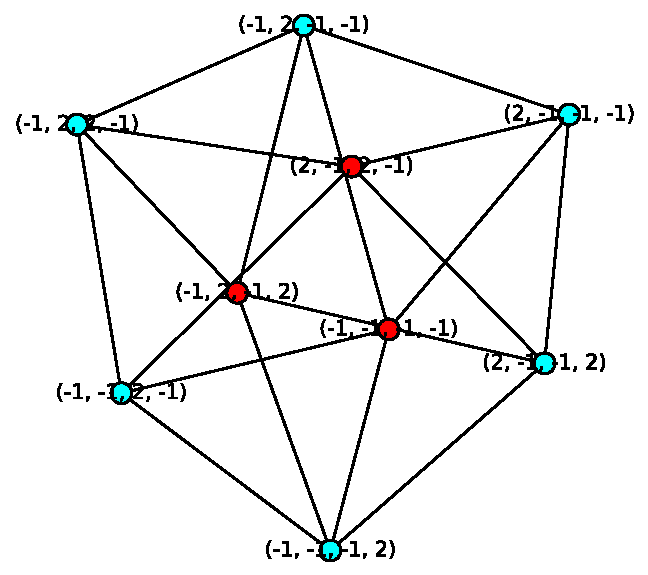
\includegraphics[scale=0.7]{./figures/grafDD.pdf}
  \caption{The edge graph of $\Delta \times \Delta$. The red vertices are the diagonal vertices $v_{ii}$.}
  \label{fig:edgegraphDD}
\end{figure}
  \todo{make nicer figure}
We want a projection sending the vertices $v_{ii}$ ($i=1,2,3$) to the origin in $\R^2$. In \cref{fig:edgegraphDD}, we have visualized the edge graph of $\Delta^2 \times \Delta^2$. The three vertices that are sent to zero are marked in red.

By demanding that $v_{12} \mapsto (1,0)$ and $v_{23} \mapsto (0,1)$, together with $v_{ii} \mapsto (0,0)$, we get a system of $8$ linear equations, corresponding to a unique map $\R^4 \to \R^2$ with the required properties. We get:

\[
A'^T =  \frac 13
\begin{pmatrix}
0 & 1 & 0 & -1 \\
-1 & 0 & 1 & 0
\end{pmatrix}.
\]
The image generates a sublattice $\frac 13 \Z^2 \subset \Z^2$. Replace $A'$ by $A \stackrel{\Delta}{=} 3A'$, and consider only the sublattice.

The images of the rays of the fan of $\dP6$ under $A^T$ are exacty the $6$ rays of the fan of $\P^2 \times \P^2$. This means that the map $C^T$ in the Lemma is the identity matrix $I_6$, and we have a diagram
\[
\begin{tikzcd}
0 \arrow{r} &  \Z^4 \arrow{r}{R_1} \arrow{d}{A^T} & \Z^6 \arrow{d}{I_6} \arrow{r} & \Pic(\P^2 \times \P^2)=\Z^2  \arrow{d}{i^\ast} \arrow{r} & 0\\
0 \arrow{r} &  \Z^2 \arrow{r}{R_2} & \Z^{6} \arrow{r} & \Pic(\dP6)=\Z^4 \arrow{r} & 0
\end{tikzcd}
\]
It now follows from the snake lemma that $i^\ast$ is injective with zero cokernel.
\end{example}

This lemma let us compute explicitly what the induced map of Picard groups is using only the toric data.

\begin{theorem}
The two affine smoothings are topologically different. The homology groups are:
\begin{center}
\begin{tabular}{ l | >{$}c<{$}  >{$}c<{$}  >{$}c<{$}  >{$}c<{$}  >{$}c<{$}  >{$}c<{$}  >{$}c<{$} | c }
 Group & 1 & 1 & 2 & 3 & 4 & 5 & 6 & Euler characteristic \\
\hline
$H^i(X_1,\Z)$ & 1 & 0 & 2 & 1 & 0 & 0 & 0 & 2 \\
$H^i(X_2,\Z)$ & 1 & 0 & 1 & 2 & 0 & 0 & 0  & 0
\end{tabular}
\end{center}
\end{theorem}

\begin{proof}
The singular cohomology of $M=\P^1 \times \P^1 \times \P^1$ is given by $(1,0,3,0,3,0,1)$, which can be computed by the Künneth formula (see \cite{hatcher_topology}, page 275). The cohomology of $\dP6$ is given by $(1,0,4,0,1)$.

We will use the Lefschetz duality theorem \cite{spanier_topology}, which in this case says that $H_q(M \bs dP_6; \Z) \simeq H^{6-q}(M,dP_6;\Z)$. The long exact sequence of the pair $(M,\dP6)$ (\cite{hatcher_topology}, page 200) takes the form:

\begin{center}
\begin{tikzpicture}[descr/.style={fill=white,inner sep=1.5pt}]
        \matrix (m) [
            matrix of math nodes,
            row sep=1em,
            column sep=2.5em,
            text height=1.5ex, text depth=0.25ex
        ]
        { 0 & H^0(M,D;\Z) & \Z & \Z \\
            & H^1(M,D;\Z) & 0 & 0 \\
            & H^2(M,D;\Z) & \Z^3 & \Z^4 \\
            & H^3(M,D;\Z) & 0 & 0 \\
            & H^4(M,D;\Z) & \Z^3 & \Z \\
            & H^5(M,D;\Z) & 0 & 0 \\
            & H^6(M,D;\Z) & \Z & 0 \\
        };

        \path[overlay,->, font=\scriptsize,>=latex]
        (m-1-1) edge (m-1-2)
        (m-1-2) edge (m-1-3)
        (m-1-3) edge (m-1-4)
        (m-1-4) edge[out=355,in=175] node[descr,yshift=0.3ex] {$\delta$} (m-2-2)
        (m-2-2) edge (m-2-3)
        (m-2-3) edge (m-2-4)
        (m-2-4) edge[out=355,in=175] node[descr,yshift=0.3ex] {$\delta$} (m-3-2)
        (m-3-2) edge (m-3-3)
        (m-3-3) edge (m-3-4)
        (m-3-4) edge[out=355,in=175] node[descr,yshift=0.3ex] {$\delta$} (m-4-2)
        (m-4-2) edge (m-4-3)
        (m-4-3) edge (m-4-4)
        (m-4-4) edge[out=355,in=175] node[descr,yshift=0.3ex] {$\delta$} (m-5-2)
        (m-5-2) edge (m-5-3)
        (m-5-3) edge (m-5-4)
        (m-5-4) edge[out=355,in=175] node[descr,yshift=0.3ex] {$\delta$} (m-6-2)
        (m-6-2) edge (m-6-3)
        (m-6-3) edge (m-6-4)
        (m-6-4) edge[out=355,in=175] node[descr,yshift=0.3ex] {$\delta$} (m-7-2)
        (m-7-2) edge (m-7-3)
        (m-7-3) edge (m-7-4);
\end{tikzpicture}
\end{center}

From the exactness of the sequence, we immediately find $H^0(X_1;\Z)=\Z$. Also, since $H^0(M;\Z) \to H^0(\dP6;\Z)$ is an isomorpism (both are connected), it follows that $H^6(X_1;\Z)=H^5(X_1;\Z)=0$.

The other groups depend upon the explicit form of the maps $H^2(M;\Z) \to H^2(\dP6;\Z)$ and $H^4(M;\Z) \to H^4(\dP6,\Z)$.

The map $H^2(M;\Z) \to H^2(\dP6;\Z)$ can be identified with the map $i^\ast \colon \Pic(M) \to \Pic(\dP6)$ induced by the inclusion. This map was computed in \cref{example:p1p1p1}. It is an injective map with torsion-free cokernel, and it follows from the long-exact sequence and the Lefschetz theorem that $H_3(X_1;\Z) \simeq H^3(M,dP_6; \Z) \simeq \Z$, and also that $H_4(X_1;\Z)=0$.

To compute the map $H^4(M;\Z) \to H^4(\dP6;\Z)$, note that $H^4(M;\Z)$ is Poincaré dual to $H_ 2(M;\Z)$, and this group is generated by $\P^1 \times \{pt\} \times \{ pt\}$ (and permutations)\footnote{I thank the math.stackexchange user \emph{nefertiti} for this argument.}. Also, $H^4(\dP6;\Z) \simeq H_0(\dP6,\Z)=\Z$. In this description, pullback corresponds to intersection, and one sees that the map is given by $(a,b,c) \mapsto a+b+c$, since the three $\P^1$'s intersect $\dP6$ in a single point each. This map has two-dimensional kernel, and we conclude that $H_2(X_1;\Z) \simeq H^4(M,\dP6;\Z) = \Z^2$, and that $H^1(X_1;\Z)=0$.

The computations for $X_2$ are similar. We first note that the Picard group of $M=\P(\mathcal T_{\P^2})$ is generated by the pullbacks $F,G$ of the generators of $\Pic(\P^2_{x_0x_1x_2} \times \P^2_{y_0y_1y_2})$. Say $F$ is represented by $V(x_0)$ and $G$ is represented by $V(y_0)$.

Again we compute the intersections of $F$ and $G$ with $dP_6$. Intersecting with $F$ is computed by decomposing the ideal $(x_0,x_1y_0-x_2y_1,x_1y_0-x_0y_2)$ in $k[x_0,x_1,x_2,y_0,y_1,y_2]$ and saturating by $(x_0,x_1,x_2)$ and $(y_0,y_1,y_2)$. This can either be done by hand or by using \MM. Either way, we find that $\restr{F}{dP_6} = E_3+L_{23} + E_2=H$, using the notation from earlier this chapter\todo{!! not true, there is no such notation!!}. Similarly $\restr{G}{dP_6}=L_{23}+L_{12}+E_2=2H-E_1-E_2-E_3$. Hence the map on cohomology is given by the matrix

\[
H^2(M;\Z) \simeq H_4(M;\Z) \simeq \Z^2 \xrightarrow{
	\begin{pmatrix*}[r]
	0 & -1 \\
	0 & -1 \\
	0 & -1  \\
	1 & 2 
	\end{pmatrix*}
} \Z^4 \simeq H_2(\dP6;\Z) \simeq H^2(\dP6;\Z).
\]

This is an injective map, and as above, we conclude that $H_3(X_2;\Z) \simeq H^3(M,\dP6;\Z) \simeq \Z^2$, and also that $H_4(X_1;\Z)=0$.
\end{proof}

\begin{remark}
In fact, the Andreotti-Frankel theorem \cite{andreotti_affinecw} states the following: if $V$ is any smooth affine variety of complex dimension $n$, then it has the homotopy type of a CW complex of real dimension $n$. Thus it comes for free that $H^j(X_i,\Z)=0$ for $j > 3$.
\end{remark}
 